% !TeX program = pdflatex
% !TeX encoding = UTF-8
%=======================================================================
%  GRIS-NOT-001  ·  Plantilla de notas rápidas para la memoria
%  Proyecto 00503 - Generator inspection robotic system · Mecanalisis
%  Identidad: GRIS-IDENTIDAD-001 v1.4
%-----------------------------------------------------------------------
%  CÓMO USARLA (en 3 pasos)
%
%   1. Copiá este archivo con el código de la nota, en su propia carpeta:
%         memoria/notas/02489-00-MC007/02489-00-MC007.tex
%      El número (###) es correlativo: mirá la última nota y sumá uno.
%      Las figuras van en memoria/notas/02489-00-MC007/figuras/ y el PDF
%      final se copia a memoria/pdf/.
%
%   2. Completá los cuatro datos del bloque «DATOS DE LA NOTA».
%
%   3. Escribí:
%        · Resultados (obligatorio, siempre primero): lo que se sabe
%          ahora que antes no se sabía. Frases cortas, con números.
%        · El resto es libre. Usá los títulos que te sirvan, o ninguno.
%
%   Compilar desde la carpeta de la nota:  pdflatex 02489-00-MC007.tex
%   En Overleaf: subí el .tex y logo-gris.pdf.
%
%  LOGO: se usa «logo-gris.pdf» (GRIS-LOGO-003, reducido) de esta carpeta
%  o de ../../plantilla/. Si falta, se escribe «GRIS» como marcador.
%=======================================================================
\documentclass[11pt,a4paper]{article}

%=======================================================================
%  DATOS DE LA NOTA  ← lo único que hay que tocar arriba
%=======================================================================
\newcommand{\codigo}{02489-00-MC008}          % 02489-00-MC###
\newcommand{\titulo}{Selección del conector Fischer MiniMax}
\newcommand{\autor}{Matías Gaviño}
\newcommand{\fecha}{29/09/2026}                    % o p. ej. {24/09/2026}

%=======================================================================
%  ESTILO  (no hace falta tocar nada de aquí hasta \begin{document})
%=======================================================================
\usepackage[T1]{fontenc}
\usepackage[utf8]{inputenc}
\usepackage[spanish,es-noshorthands,es-tabla]{babel}
\usepackage{lmodern}
\usepackage[a4paper,top=3.0cm,bottom=2.4cm,left=2.4cm,right=2.4cm,
            headheight=20pt,headsep=1.2cm,footskip=1.1cm]{geometry}
\usepackage{microtype}
\usepackage{xcolor}
\usepackage{graphicx}
\usepackage{booktabs}
\usepackage{array}
\usepackage{enumitem}
\usepackage{titlesec}
\usepackage{fancyhdr}
\usepackage{caption}
\usepackage{amsmath,amssymb}
\usepackage{float}
\usepackage[hidelinks]{hyperref}

% --- colores -----------------------------------------------------------
\definecolor{gris-naranja}{HTML}{FF7A00}   % naranja institucional
\definecolor{tinta}{HTML}{1E2328}
\definecolor{gris-medio}{HTML}{6B7280}
\definecolor{gris-linea}{HTML}{DADDE1}
\color{tinta}

\hypersetup{pdftitle={\codigo\ -- \titulo}, pdfauthor={\autor},
            colorlinks=true, linkcolor=tinta, urlcolor=tinta}

% --- logo ---------------------------------------------------------------
\graphicspath{{./}{figuras/}{../../plantilla/}}
\newcommand{\logogris}{%
  \IfFileExists{logo-gris.pdf}
    {
\includegraphics[height=16pt]{logo-gris.pdf}}
    {\IfFileExists{../../plantilla/logo-gris.pdf}
      {
\includegraphics[height=16pt]{../../plantilla/logo-gris.pdf}}
      {{\fontsize{18}{18}\selectfont\bfseries\sffamily\color{gris-naranja}GRIS}}}}

% --- tipografía del cliente (código documental) --------------------------
% Geogrotesque no es libre; se usa Roboto Condensed Bold, que viene con
% TeX Live y Overleaf y tiene el mismo aire que el logo.
\newcommand{\fuentecliente}{\fontfamily{Roboto-TLF}\fontseries{bc}\selectfont}

% --- encabezado y pie ---------------------------------------------------
\pagestyle{fancy}
\fancyhf{}
\renewcommand{\headrulewidth}{0.4pt}
\renewcommand{\headrule}{\vspace{3pt}{\color{gris-linea}\hrule height \headrulewidth}}
\fancyhead[L]{\logogris}
\fancyhead[R]{{\fuentecliente\fontsize{12}{12}\selectfont\color{gris-medio}\codigo}}
\fancyfoot[R]{\footnotesize\color{gris-medio}\thepage}

% --- títulos numerados ----------------------------------------------------
\setcounter{secnumdepth}{2}
\titleformat{\section}{\large\bfseries}{\thesection}{0.8em}{}
\titleformat{\subsection}{\normalsize\bfseries}{\thesubsection}{0.8em}{}
\titlespacing*{\section}{0pt}{16pt}{5pt}
\titlespacing*{\subsection}{0pt}{11pt}{3pt}

% --- texto ------------------------------------------------------------------
\setlength{\parindent}{0pt}
\setlength{\parskip}{6pt}
\linespread{1.05}
\setlist{topsep=2pt, itemsep=2pt, parsep=0pt, leftmargin=1.2em}
\setlist[itemize]{label={\raisebox{0.15ex}{\small$\bullet$}}}
\captionsetup{font={small,color=gris-medio}, labelfont=bf, skip=5pt}
\renewcommand{\arraystretch}{1.25}

% --- cabecera de la nota ------------------------------------------------------
\newcommand{\cabecera}{%
  \thispagestyle{fancy}%
  {\fontsize{20}{24}\selectfont\bfseries\titulo\par}%
  \vspace{5pt}%
  {\small\color{gris-medio}\fecha\quad·\quad\autor\par}%
  \vspace{6pt}}

% --- ayudas opcionales --------------------------------------------------------
% \figura{archivo}{ancho}{pie}
\newcommand{\figura}[3]{%
  \begin{figure}[htbp]\centering
    \includegraphics[width=#2\linewidth]{#1}\caption{#3}
  \end{figure}}

%=======================================================================
\begin{document}
\cabecera

%-----------------------------------------------------------------------
%  RESULTADOS  (siempre primero, lo único obligatorio)
%  Qué se sabe ahora. Cada punto se entiende sin leer el resto.
%  Si hay un número, ponelo: «error < 2 mm», no «error bajo».
%-----------------------------------------------------------------------
\section{Resultados}
\begin{itemize}
  \item \textbf{Conjunto seleccionado:} receptáculo MR11WS08 0019 AN1 E1AP (P/N 131600, PCB, rear panel mount, bloqueo a rosca) y plug MP11ZS08 0019 AN1 Z1AS (P/N 131633, soldable, latón/PEEK). Ambos son Size 08, 19 contactos: 15 de señal de 1~A y 4 de potencia de 5~A, todos de \ensuremath{\varnothing}0,5~mm.
  \item \textbf{Corte de panel:} \ensuremath{\varnothing}10,45$^{+0,1}_{\,0}$~mm con un plano superior (cota $Y=10{,}2^{+0,1}_{\,0}$~mm). Rosca de panel M10,5$\times$0,5, tuerca ranurada con llave de 10~mm, par 1,5~N\,m.
  \item \textbf{Robustez verificada en los datasheets:} IP68, $-40$ a $+135$~°C, 5\,000 ciclos, vibración 10--2\,000~Hz a 15~g (solo versión a rosca), choque 300~g, niebla salina 1\,000~h, blindaje 360°. Plug a rosca: \ensuremath{\varnothing}12,9~mm.
  \item \textbf{Potencia 48~V:} viable. La tensión asignada de esta configuración es $\le$100~V (no 250~V; ese valor es de la variante USB de 9 contactos), suficiente para 48~V con margen 2,1$\times$.
  \item \textbf{Límite real: caída en el cable.} Con 2$\times$AWG24 por polaridad el lazo vale $\approx$0,086~$\Omega$/m. Para $\Delta V\le 5$\,\% (2,4~V) la corriente continua máxima es \textbf{2,8~A a 10~m} y \textbf{1,9~A a 15~m}. A 3~A y 10~m llegan 45,4~V y el cable disipa 7,7~W.
  \item \textbf{Discrepancia sobre Ethernet:} la especificación técnica (p.~J-4) marca Ethernet (5~Gbit/s, AWG24) solo para el Size 08 de \emph{8 contactos}. Para el de 19 contactos marca audio/vídeo 10,2~Gbit/s\textsuperscript{*} y USB~2.0, no Ethernet. Fischer \emph{sí} recomienda en J-18 los pares 8/19, 10/11, 13/14 y 16/17 para Ethernet en el de 19, pero no publica validación 1000BASE-T. No hallé «Ethernet 10~Gbit/s con AWG28» en el documento.
  \item \textbf{Pendiente:} (i) corriente continua real del robot; (ii) confirmar por escrito con Fischer la validación 1000BASE-T en el 19 contactos; (iii) confirmar el significado de $E_{\max}=2{,}3$~mm (¿espesor de panel útil?); (iv) diseño de pistas de 5~A en la PCB con pines de \ensuremath{\varnothing}0,4~mm.
\end{itemize}

\section{Conjunto seleccionado}
\begin{table}[H]\centering
  \caption{Referencias del conjunto (datasheets de Fischer).}
  \begin{tabular}{l l l}
    \toprule
    & Receptáculo & Plug del cable \\
    \midrule
    P/N & 131600 & 131633 \\
    Designación & MR11WS08 0019 AN1 E1AP & MP11ZS08 0019 AN1 Z1AS \\
    Descripción & Panel rear mounted, front-projecting & Cable mounted \\
    Terminación & PCB (pin \ensuremath{\varnothing}0,4~mm) & Soldadura (máx. AWG24) \\
    Bloqueo & Screw-locking & Screw-locking, código 1 \\
    Material & Latón antracita, PEEK & Latón antracita, PEEK \\
    Contactos & 15$\times$1~A + 4$\times$5~A & 15$\times$1~A + 4$\times$5~A \\
    Ensayo (mated) & \multicolumn{2}{c}{0,9~kV\,CA c/masa y c/c; 1,5 / 1,2~kV\,CC} \\
    \bottomrule
  \end{tabular}
\end{table}

\begin{figure}[H]\centering
  \begin{minipage}{0.46\linewidth}\centering
    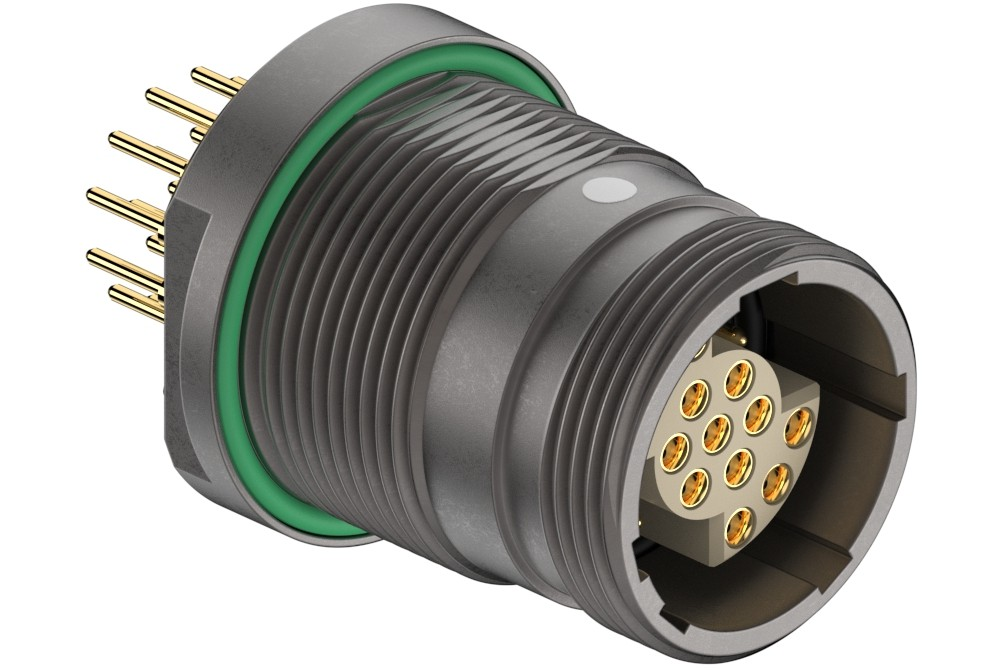
\includegraphics[width=\linewidth]{mr11ws08_0019_an1_e1ap.jpg}\\[2pt]{\small (a) Receptáculo 131600}
  \end{minipage}\hfill
  \begin{minipage}{0.46\linewidth}\centering
    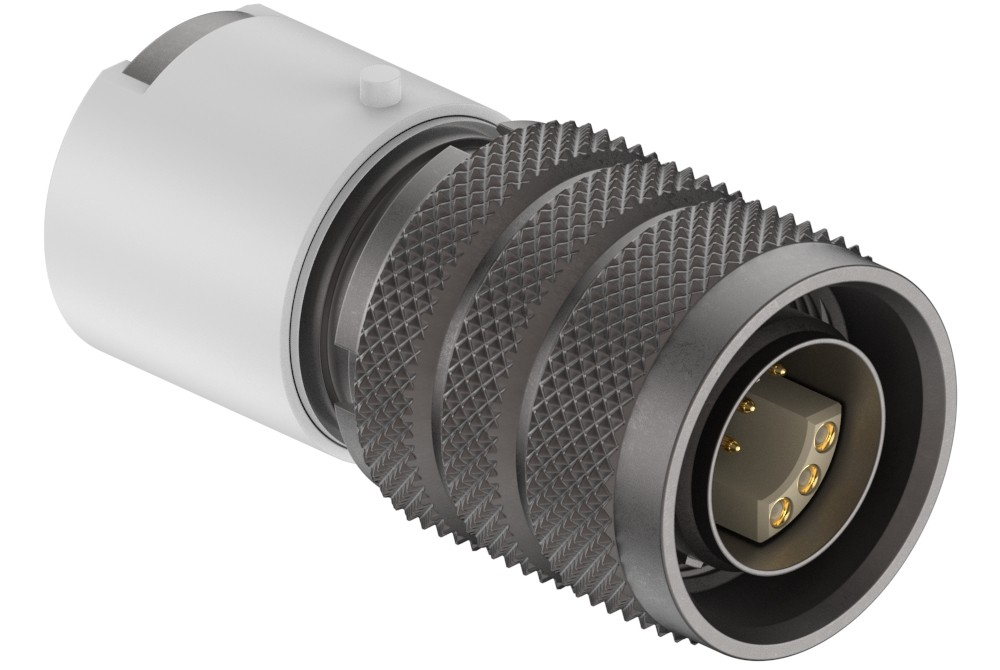
\includegraphics[width=\linewidth]{mp11zs08_0019_an1_z1as.jpg}\\[2pt]{\small (b) Plug 131633}
  \end{minipage}
  \caption{Elementos seleccionados (imágenes del catálogo online de Fischer).}
\end{figure}

\section{Corte de panel}
El receptáculo MR11-S (tabla J-15 de la especificación técnica) exige un agujero circular con un plano en la parte superior. Se fija con una tuerca ranurada M10,5$\times$0,5 (llave 10~mm, par 1,5~N\,m); el datasheet 131600 declara \ensuremath{\varnothing}10,45~mm de corte.

\begin{figure}[H]\centering
  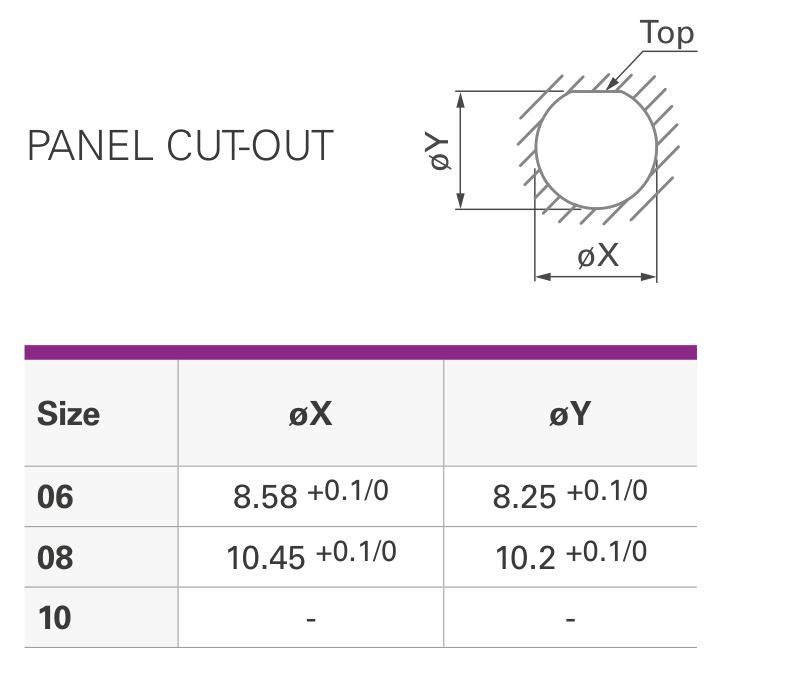
\includegraphics[width=0.62\linewidth]{panelcut_oficial.png}
  \caption{Corte de panel, captura de la tabla J-15 (Fischer, Technical Specification Vol.~2 MiniMax).}
\end{figure}

\begin{figure}[H]\centering
  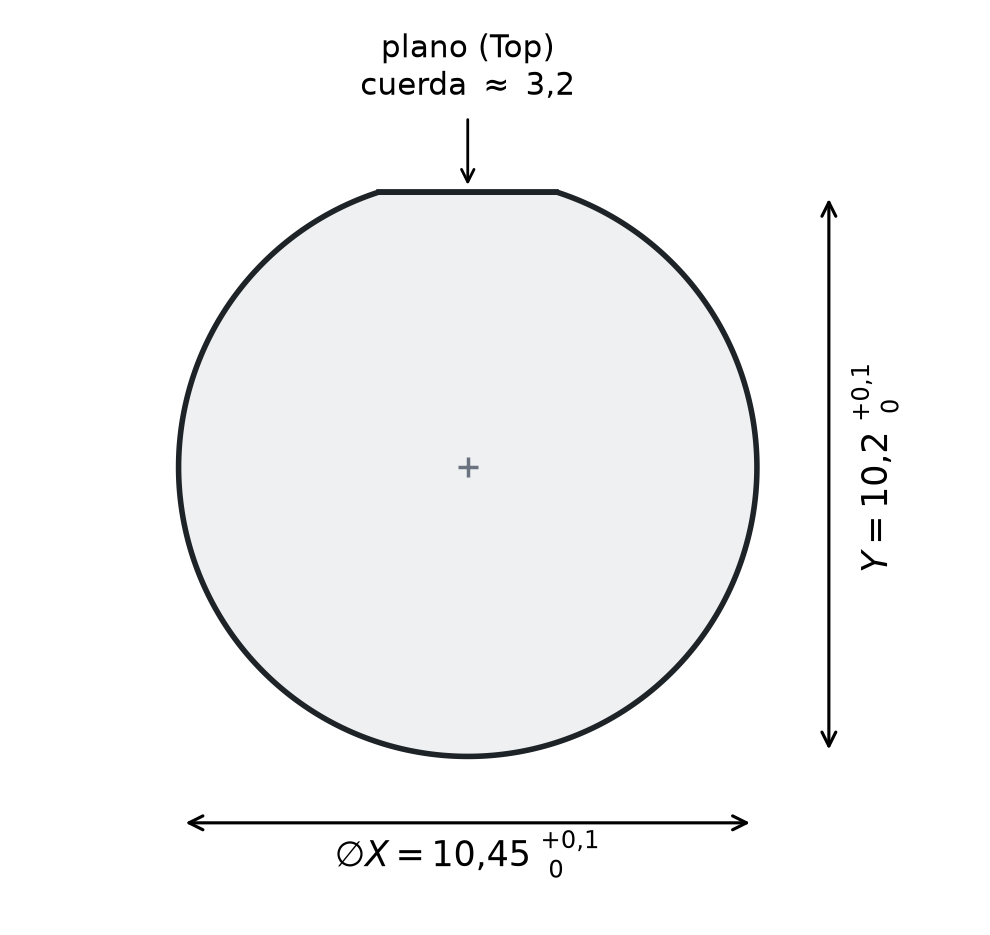
\includegraphics[width=0.55\linewidth]{corte_panel.png}
  \caption{Corte de panel Size 08 redibujado a partir de la figura oficial. La cuerda del plano ($\approx$3,2~mm) no figura en Fischer: se deduce geométricamente de $X$ e $Y$ ($\approx$ estimado).}
\end{figure}

\begin{table}[H]\centering
  \caption{Dimensiones del MR11-S Size 08, contacto PCB (mm; J-15).}
  \begin{tabular}{l r l r}
    \toprule
    \ensuremath{\varnothing} D1 (cuello) & 12,0 & Rosca de panel M1 & M10,5$\times$0,5 \\
    \ensuremath{\varnothing} D2 (MR12) & 13,7 & Rosca de bloqueo M2 & M10$\times$2 \\
    A & 7,3 & Longitud total L & 18,8 \\
    B (pines PCB) & 4,7 & $E_{\max}$ & 2,3 \\
    \bottomrule
  \end{tabular}
\end{table}

\begin{figure}[H]\centering
  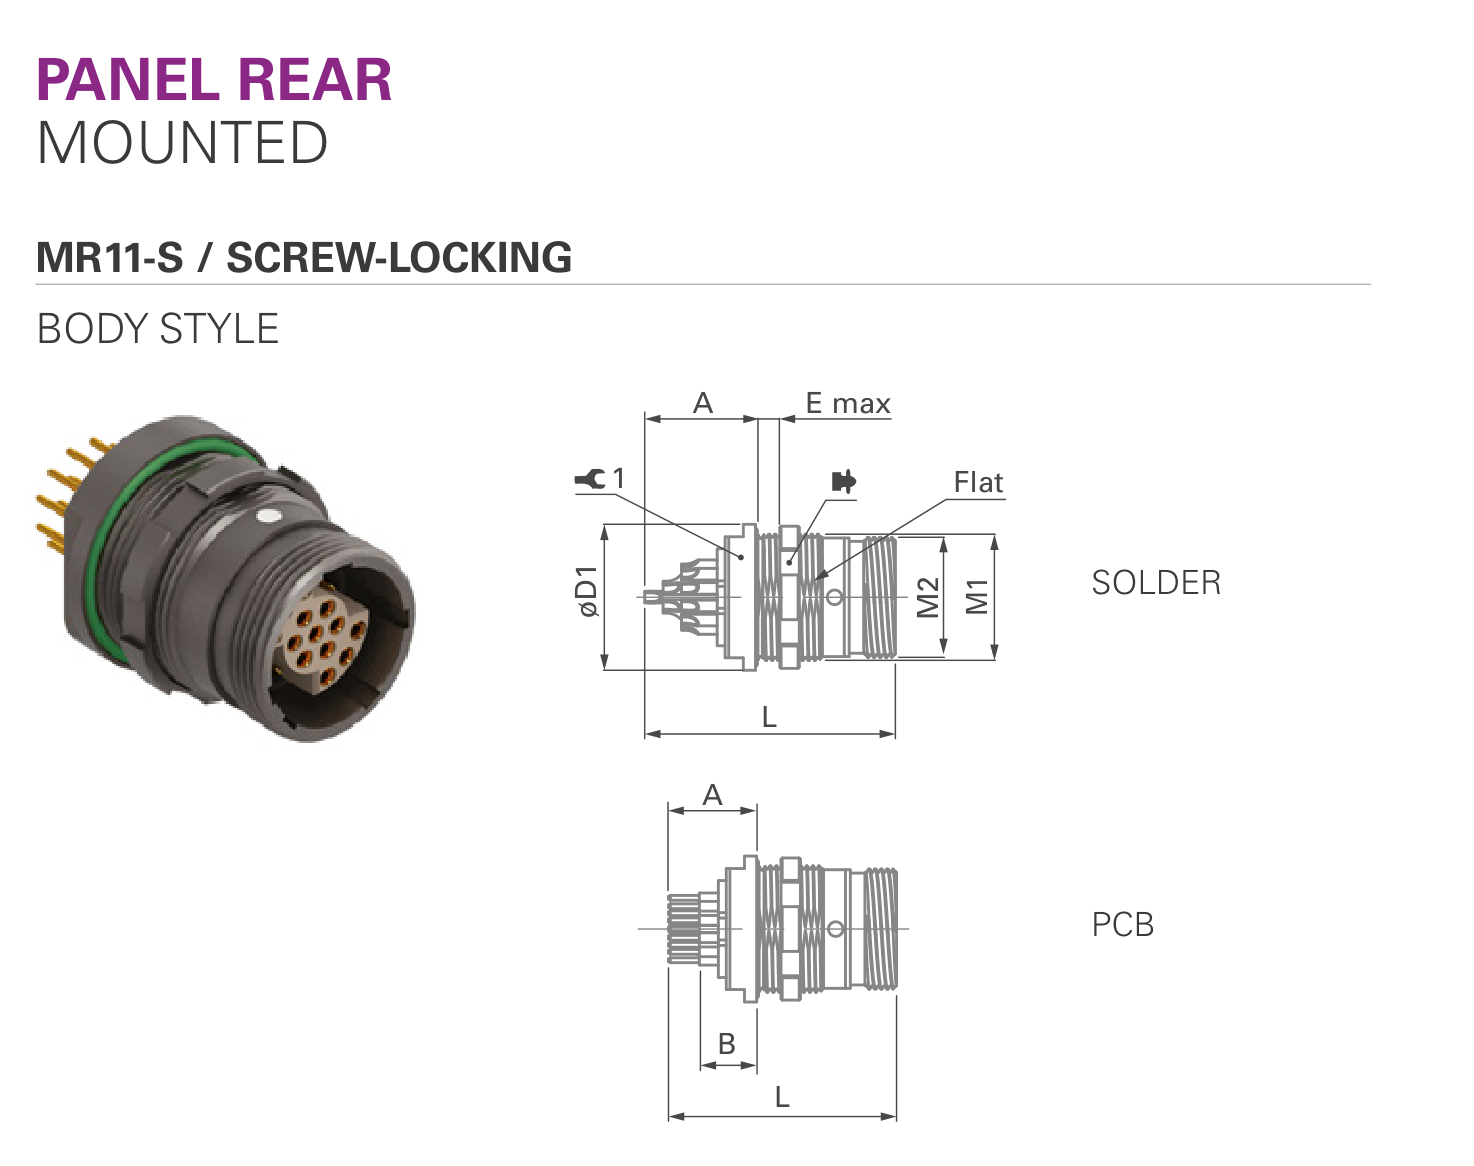
\includegraphics[width=0.7\linewidth]{mr11s_dibujo.png}
  \caption{Plano del receptáculo MR11-S (catálogo Fischer, J-15). Abajo, versión PCB.}
\end{figure}

\section{Plug y sobremoldeado}
\begin{figure}[H]\centering
  \begin{minipage}[c]{0.45\linewidth}\centering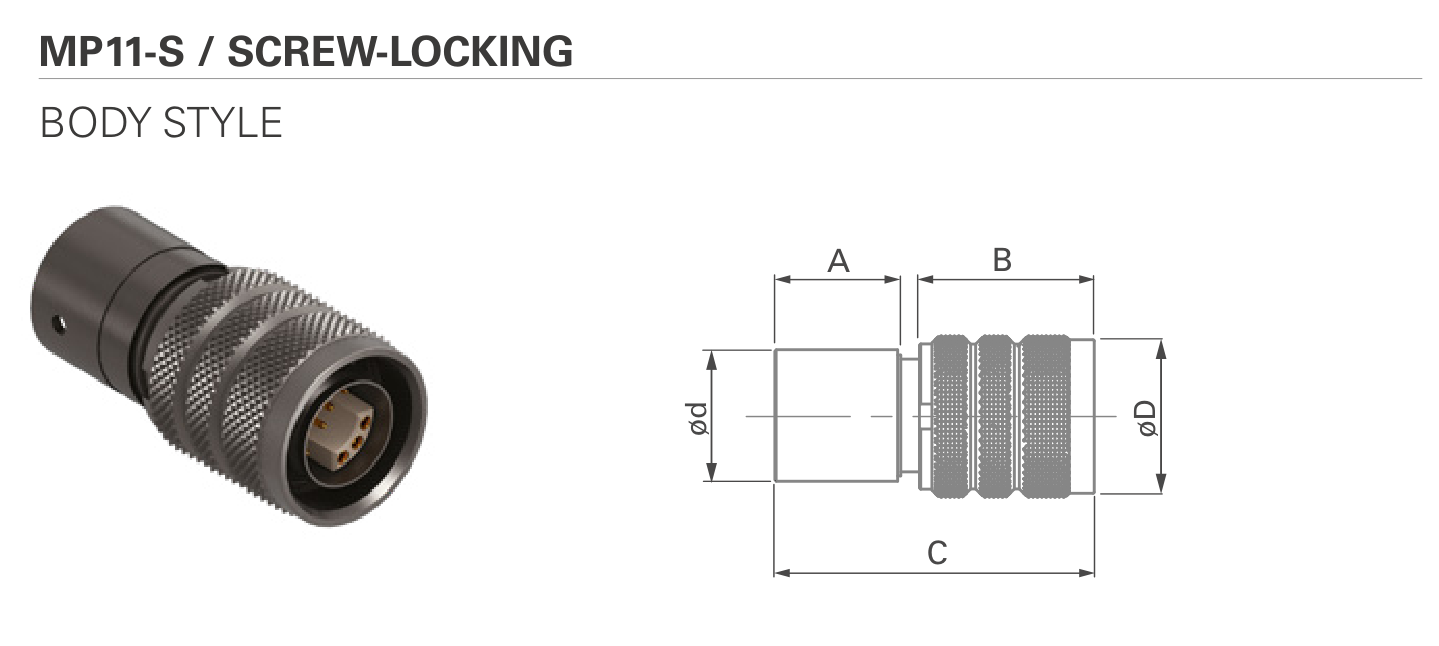
\includegraphics[width=\linewidth]{mp11s_dibujo.png}\end{minipage}\hfill
  \begin{minipage}[c]{0.5\linewidth}\centering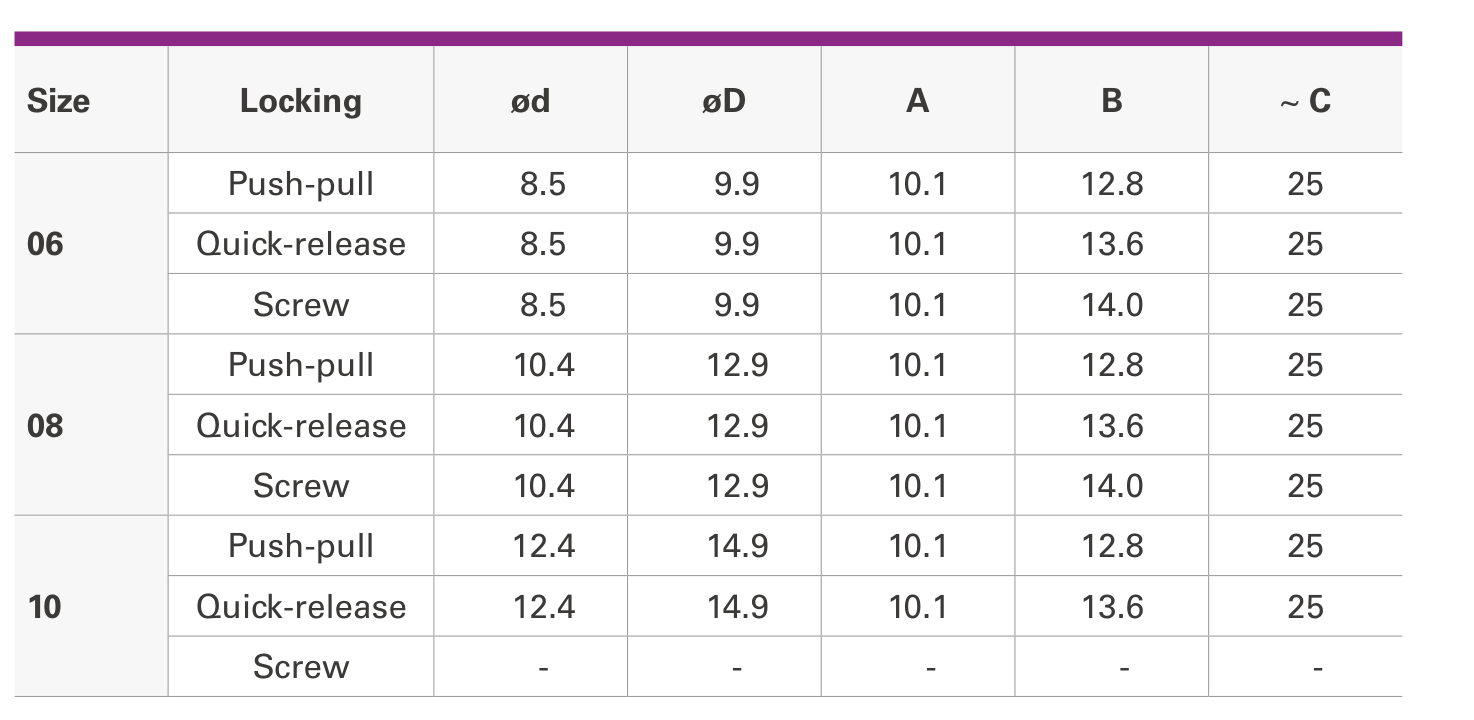
\includegraphics[width=\linewidth]{mp11s_tabla.png}\end{minipage}
  \caption{Plug MP11-S a rosca (J-8): \ensuremath{\varnothing} D=12,9~mm, longitud $\approx$25~mm, $\ensuremath{\varnothing} d$=10,4~mm.}
\end{figure}
\begin{figure}[H]\centering
  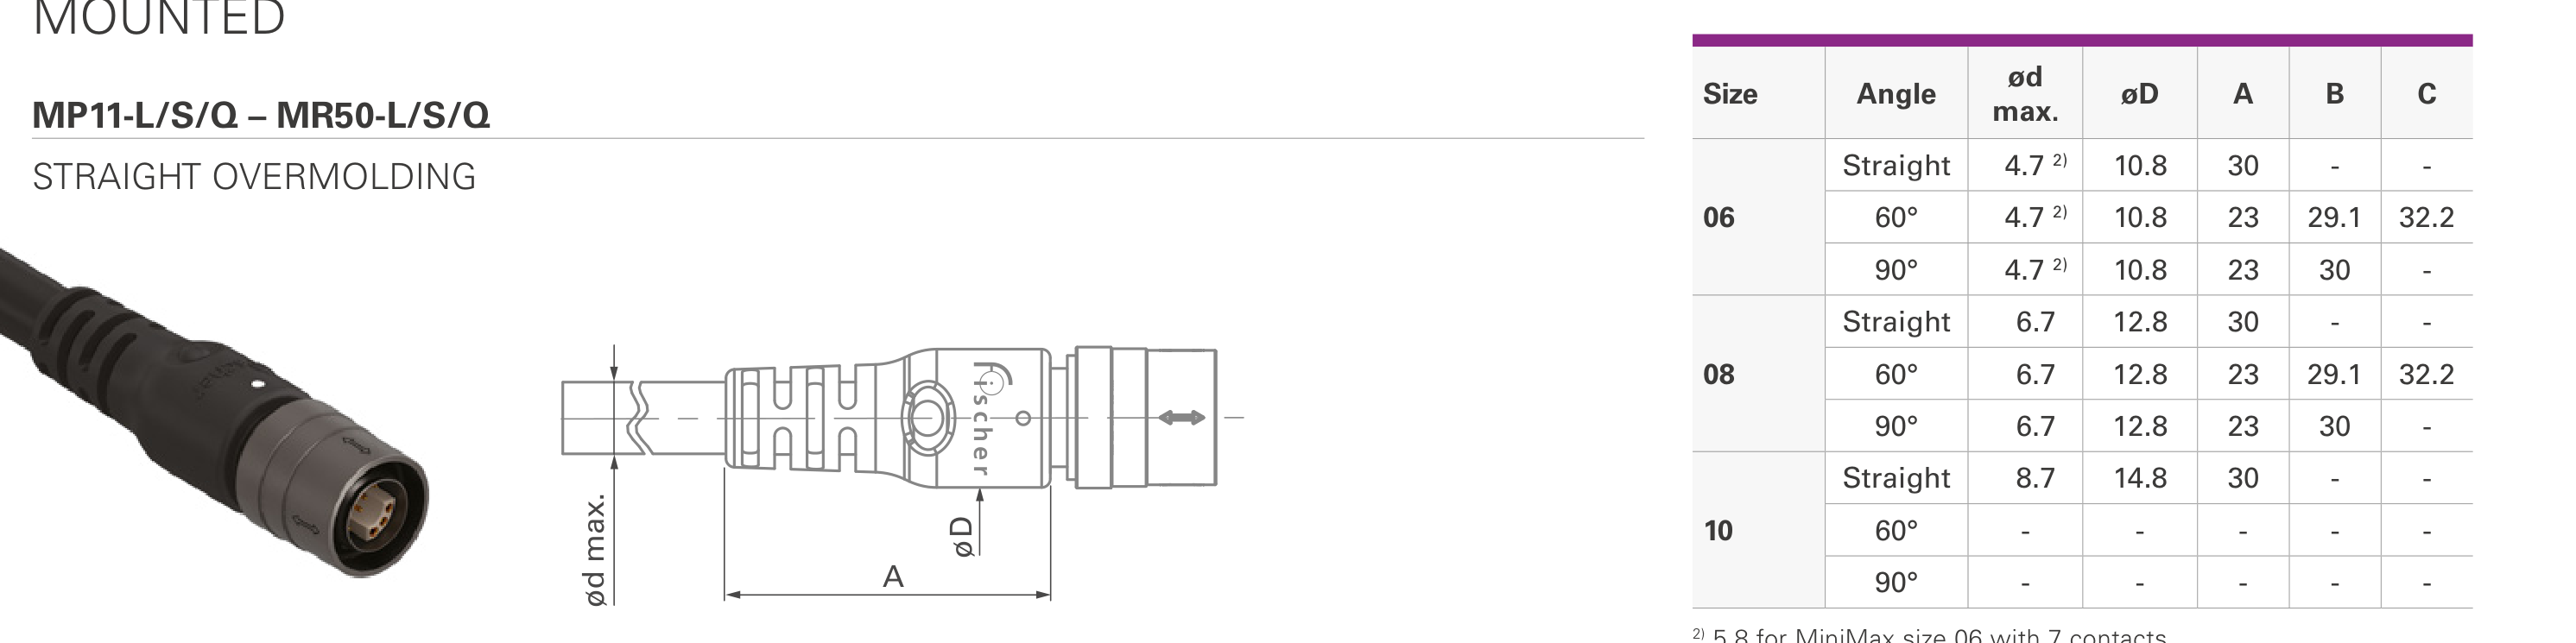
\includegraphics[width=\linewidth]{overmolding.png}
  \caption{Sobremoldeado (J-9): Size 08, cable máx. \ensuremath{\varnothing}6,7~mm, \ensuremath{\varnothing}12,8~mm, largo 30~mm (recto); a 90° y 60° bajo pedido.}
\end{figure}

\section{Distribución de contactos}
\begin{figure}[H]\centering
  \begin{minipage}[c]{0.27\linewidth}\centering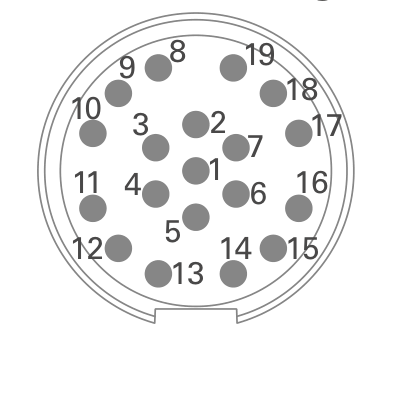
\includegraphics[width=\linewidth]{pinout_19.png}\end{minipage}\hfill
  \begin{minipage}[c]{0.68\linewidth}\centering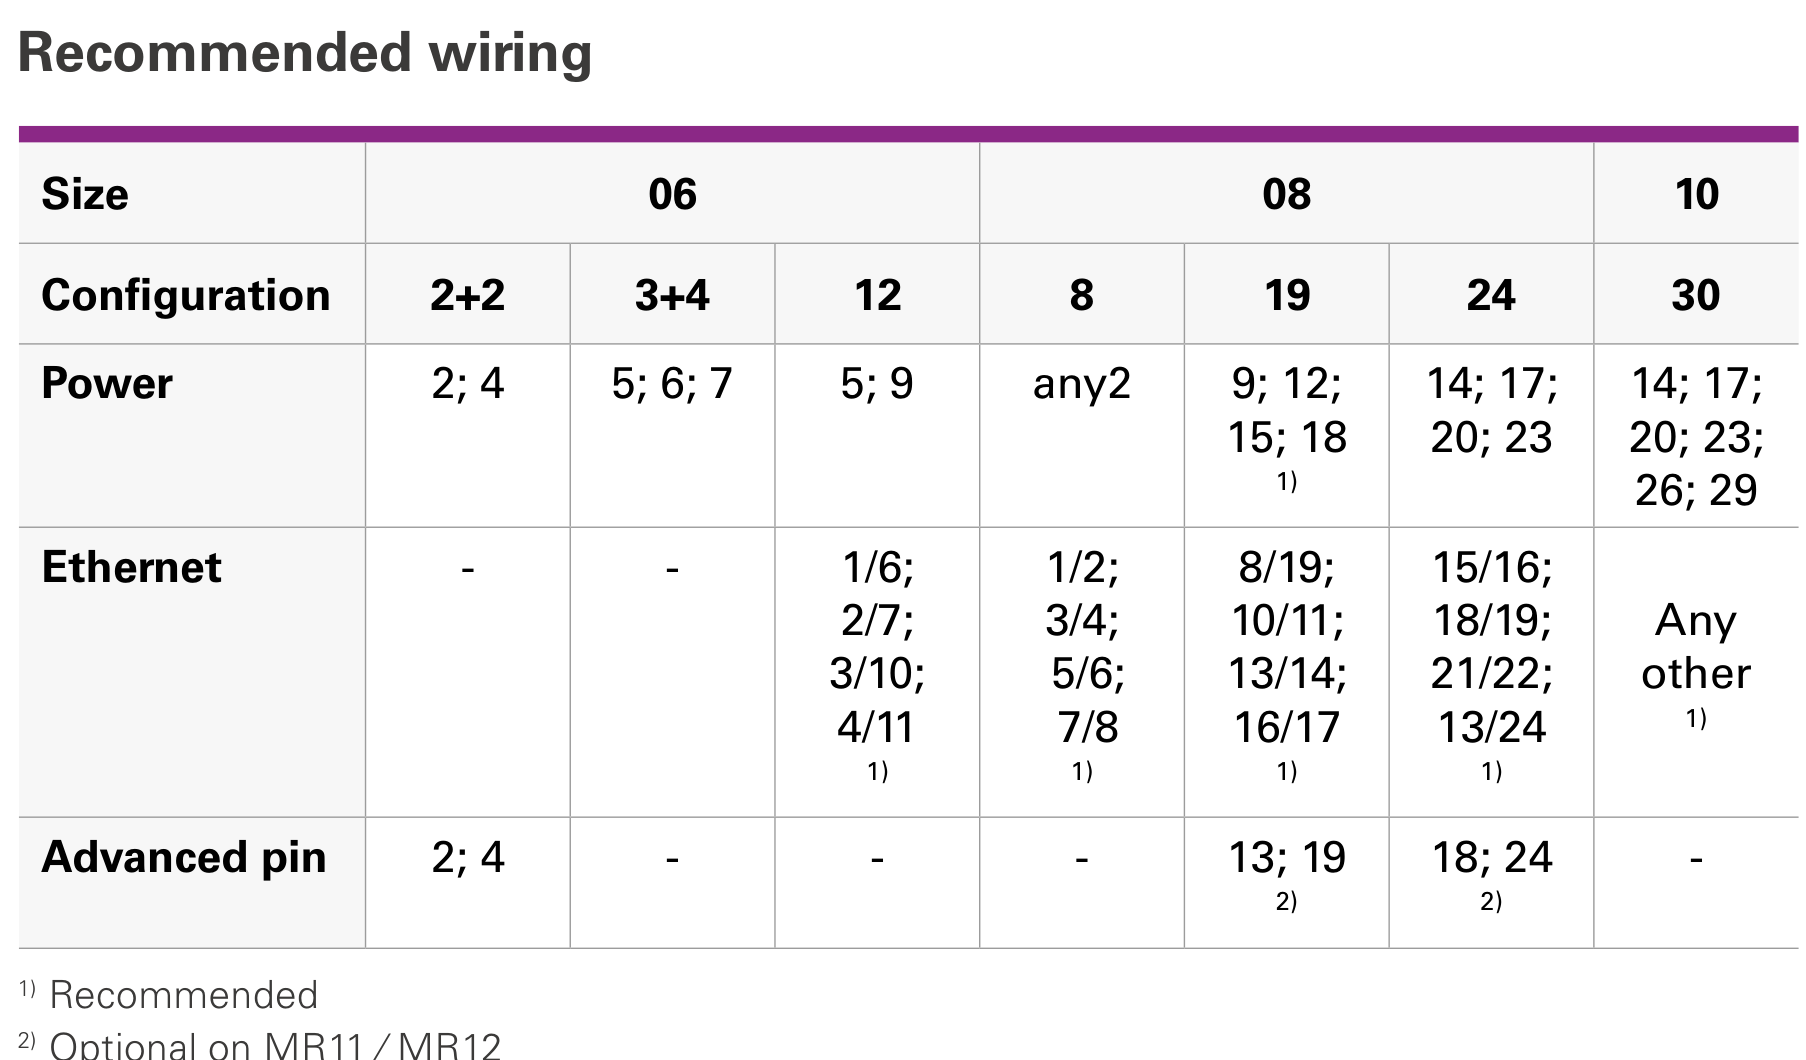
\includegraphics[width=\linewidth]{cableado_rec.png}\end{minipage}
  \caption{Izq.: numeración de los 19 contactos (vista de frente, J-18). Der.: cableado recomendado por Fischer (potencia 9/12/15/18; Ethernet 8/19, 10/11, 13/14, 16/17).}
\end{figure}

\begin{table}[H]\centering
  \caption{Asignación propuesta.}
  \begin{tabular}{l l}
    \toprule
    Pines & Función \\
    \midrule
    8--19, 10--11, 13--14, 16--17 & GbE, pares 1 a 4 (recomendación J-18) \\
    9 + 12 & +48~V \\
    15 + 18 & 0~V \\
    1--2 & RS-485 A/B \\
    3--4 & Analógica diferencial +/$-$ \\
    5, 6, 7 & Reserva / RS-485 COM / referencia analógica \\
    \bottomrule
  \end{tabular}
\end{table}

Se usan los 8 conductores de 1000BASE-T, 4 contactos de potencia y quedan 3 auxiliares. Los pares Ethernet quedan en el anillo exterior, entre los contactos de potencia: hay que pedir al ensamblador que mantenga el balance del par y el blindaje del par hasta el contacto.

\begin{figure}[H]\centering
  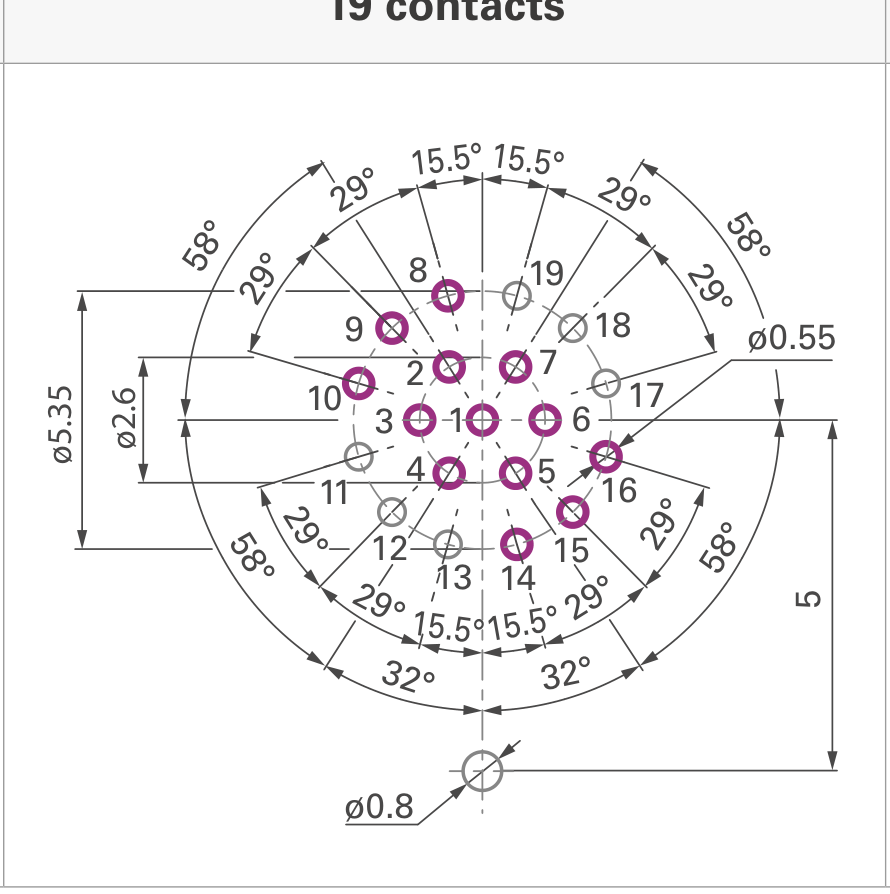
\includegraphics[width=0.55\linewidth]{pcb_layout.png}
  \caption{Disposición de agujeros en PCB, 19 contactos (J-20): pines en \ensuremath{\varnothing}0,55~mm, agujero de referencia \ensuremath{\varnothing}0,8~mm.}
\end{figure}

\section{Alimentación de 48~V y caída en el cable}
\begin{table}[H]\centering
  \caption{Datos y supuestos.}
  \begin{tabular}{p{5.4cm} p{4.6cm} p{4.6cm}}
    \toprule
    Dato & Valor & Origen \\
    \midrule
    Corriente por contacto de potencia & 5~A ($\Delta T=40$~K) & Fischer J-16, curva básica \\
    Conductor máx. en contactos & AWG24 (\ensuremath{\varnothing}0,70~mm) & Fischer J-16 \\
    Resistencia de contacto & 5~m$\Omega$ típ. & Fischer J-27 \\
    Resistividad AWG24 & 0,0858~$\Omega$/m (25~°C) & \textbf{supuesto} (tabla de cobre) \\
    Reparto de corriente & 2 conductores por polaridad, igual reparto & \textbf{supuesto} \\
    \bottomrule
  \end{tabular}
\end{table}
Lazo: $R=2\,(R_{24}/2)\,L=R_{24}L\approx0{,}086\,L$~$\Omega$ (con $L$ en m), más $\approx$5~m$\Omega$ de los cuatro contactos, despreciable. Pérdida $P=I^2R$.

\begin{table}[H]\centering
  \caption{Caída de tensión, tensión en el robot ($V_0=48$~V) y disipación en el cable (calculo.py).}
  \begin{tabular}{r r r r r r r}
    \toprule
    $I$ [A] & $\Delta V_{10}$ [V] & $V_{robot,10}$ & $P_{10}$ [W] & $\Delta V_{15}$ [V] & $V_{robot,15}$ & $P_{15}$ [W] \\
    \midrule
    2 & 1,73 & 46,3 & 3,4 & 2,58 & 45,4 & 5,1 \\
    3 & 2,59 & 45,4 & 7,7 & 3,88 & 44,1 & 11,6 \\
    4 & 3,45 & 44,5 & 13,7 & 5,17 & 42,8 & 20,6 \\
    5 & 4,31 & 43,7 & 21,4 & 6,46 & 41,5 & 32,2 \\
    10 & 8,63 & 39,4 & 85,8 & 12,9 & 35,1 & 128,7 \\
    \bottomrule
  \end{tabular}
\end{table}

Los valores de 10 y 15~m coinciden con los de la nota de partida (diferencias $\le$0,03~V por usar 0,0858 en vez de 0,086 y sumar contactos). Con el cobre a 60~°C la caída sube $\approx$14\,\%. Corriente máxima para $\Delta V\le 5$\,\% de 48~V: 2,8~A (10~m) y 1,9~A (15~m).

\section{Ethernet}
\textbf{Qué dice Fischer.} La especificación técnica (J-4) marca Ethernet solo en el Size 08 de 8 contactos, con AWG24 y 5~Gbit/s. En la fila del Size 08 de 19 contactos marca audio/vídeo (10,2~Gbit/s, «dependiente de la aplicación») y USB~2.0. El cableado recomendado (J-18) sí define cuatro pares Ethernet en el de 19 contactos. Por eso la nota de partida es correcta en la asignación de pines, pero la afirmación de que el documento contempla «Ethernet de 10~Gbit/s con AWG28» en el de 19 contactos no se pudo verificar. \textbf{No se encontró validación 1000BASE-T del 19 contactos.}

Recomendaciones:
\begin{itemize}
  \item Pedir a Fischer confirmación escrita, o un ensayo, de 1000BASE-T sobre el conjunto de 19 contactos.
  \item Mantener en la solicitud al ensamblador: \emph{«1000BASE-T verified end-to-end over complete cable assembly, including both MiniMax terminations»}.
  \item Alternativa de reducción de riesgo: Size 08 de 8 contactos para Ethernet, con la contra-parte de potencia y RS-485 en otro conector.
\end{itemize}

\section{Cable, ensamblado y proveedores}
\begin{itemize}
  \item \textbf{Construcción:} 4 pares AWG28 de 100~$\Omega$ (Ethernet), 1 par AWG28 (RS-485), 1 par AWG28 (analógica), 4$\times$AWG24 (potencia), blindaje general 360° al cuerpo. \textbf{Objetivo OD $\le$ 6,7~mm} (máximo de sobremoldeado, J-9). Una estimación por áreas (12 conductores de $\approx$0,5~mm y 4 de $\approx$0,9~mm con 60\,\% de empaquetado) da un núcleo de $\approx$3,2~mm; con blindaje y cubierta $\approx$5~mm (\emph{estimación}, a confirmar por el ensamblador).
  \item \textbf{Ensamblado por proveedor:} Fischer garantiza IP64 para cableados estándar; IP68 bajo pedido. El soldado, el destrenzado de pares, la continuidad de pantalla, el alivio de tracción y el sobremoldeado dependen del proceso.
  \item \textbf{Proveedores a consultar:} Fischer Connectors (cable assemblies), RODAN Technologies (socio oficial) y NAV Engineering.
  \item \textbf{Longitud:} 10~m preferida frente a 15~m (ver caída de tensión).
\end{itemize}

\section{Precio}
Mouser Canadá (nota de partida, sin reverificar): receptáculo CAD 288,20/u., CAD 244,99 a 10~u. El plug terminado y el cable especial requieren cotización.

\section{Limitaciones}
\begin{itemize}
  \item \textbf{Corriente real desconocida:} las conclusiones sobre 10 vs.\ 15~m dependen de ella.
  \item \textbf{Reparto de corriente:} se supuso igual entre los dos AWG24 de cada polaridad; una diferencia de resistencia de contacto lo cambia. Conviene comprobar con el ensamblador.
  \item \textbf{Derating:} los 5~A por contacto corresponden a $\Delta T=40$~K (J-16); para servicio continuo se debe aplicar el factor de reducción de Fischer (pág.~A-12, no incluida en el archivo consultado).
  \item \textbf{PCB:} cuatro pines de \ensuremath{\varnothing}0,4~mm llevan hasta 5~A cada uno; el ancho de pista y el cobre deben verificarse.
  \item \textbf{Fuentes:} catálogo online Product Finder de Fischer Connectors, consultado el 29/09/2026. Los precios no fueron reverificados.
\end{itemize}

\section{Documentos asociados}
Guardados en \texttt{fuentes/} de la nota:
\begin{itemize}
  \item Especificación técnica Fischer MiniMax, Vol.~2 (22 págs.).
  \item Datasheet del receptáculo P/N 131600.
  \item Datasheet del plug P/N 131633.
  \item Flyer de la serie MiniMax.
\end{itemize}

\end{document}
